\documentclass{article}

% Recommended packages
\usepackage{microtype}
\usepackage{graphicx}
\usepackage{subcaption}
\usepackage{booktabs}
\usepackage{hyperref}

% ICML 2026 style (blind submission)
\usepackage{icml2026}

\usepackage{amsmath,amssymb,amsfonts}
\usepackage{xcolor}
\usepackage{pgfplots}
\usepackage{tikz}
\usepackage{multirow}
\usepackage{enumitem}

\pgfplotsset{compat=1.18}

% Custom colors
\definecolor{samplingblue}{RGB}{31,119,180}
\definecolor{verbalizedred}{RGB}{214,39,40}
\definecolor{perfectgreen}{RGB}{44,160,44}
\definecolor{lightgray}{RGB}{220,220,220}
\definecolor{bingray}{RGB}{180,180,180}

\hypersetup{
  colorlinks=true,
  linkcolor=blue!60!black,
  citecolor=blue!60!black,
  urlcolor=blue!60!black
}

% Compact lists
\setlist{nosep,leftmargin=*}

\begin{document}

\twocolumn[
\icmltitle{Mind the Gap: Measuring the Calibration Disconnect Between\\Internal and Expressed Confidence in Code Language Models}

\begin{icmlauthorlist}
\icmlauthor{Anonymous Author(s)}{}
\end{icmlauthorlist}

\vskip 0.3in
]

\printAffiliationsAndNotice{}

% ============================================================
% ABSTRACT
% ============================================================
\begin{abstract}
AI coding assistants present all generated code with equal certainty, leaving developers unable to calibrate their trust. We systematically measure the gap between \emph{internal} confidence (sampling consistency across multiple generations) and \emph{expressed} confidence (verbal self-assessment) in code language models. Evaluating Qwen2.5-Coder-7B-Instruct on HumanEval (164 problems, 10 samples each), we find that sampling-based confidence is near-perfectly calibrated (ECE\,=\,0.021, AUROC\,=\,0.990), while verbalized confidence is essentially random as a correctness predictor (ECE\,=\,0.090, AUROC\,=\,0.546). The model assigns maximum self-rated confidence to 63\% of problems, yet only 87.4\% of those are actually correct. On MBPP, verbalized ECE reaches 0.755, a 63$\times$ degradation over sampling ECE. These results reveal a stark calibration disconnect: code LLMs possess reliable internal uncertainty signals but cannot communicate them. We discuss implications for the design of human-centered coding agents and present preliminary results on confidence-calibrated supervised fine-tuning.
\end{abstract}

% ============================================================
% 1. INTRODUCTION
% ============================================================
\section{Introduction}
\label{sec:intro}

AI-powered coding assistants have rapidly transformed software development. Tools such as GitHub Copilot, Cursor, and autonomous agents built on models like GPT-4, Claude, and open-source code LLMs now generate substantial fractions of production code~\citep{peng2023impact}. These systems achieve impressive pass rates on benchmarks: the model evaluated in this work, Qwen2.5-Coder-7B-Instruct~\citep{hui2024qwen25coder}, achieves pass@1\,=\,0.854 on HumanEval~\citep{chen2021evaluating}.

Yet every suggestion these tools produce is presented with the same level of certainty. A trivially correct helper function and a subtly buggy recursive algorithm receive identical visual treatment in the developer's IDE. This uniformity creates a fundamental barrier to effective human-agent collaboration: developers have no principled way to decide when to accept generated code at face value and when to scrutinize it carefully~\citep{vaithilingam2022expectation, mozannar2024reading}.

The trust calibration literature from human-computer interaction establishes that displaying AI confidence can improve human decision-making, but \emph{only when that confidence is well-calibrated}~\citep{yin2019understanding, zhang2020effect}. Poorly calibrated confidence can actively harm trust by encouraging overreliance on incorrect outputs~\citep{rechkemmer2022confidence, bansal2021does}. This motivates a critical empirical question: can code LLMs reliably express their uncertainty in words?

In this paper, we provide the first systematic comparison of \emph{internal} confidence (measured by sampling consistency) and \emph{expressed} confidence (measured by verbal self-assessment) in code language models. Our key finding is a striking calibration disconnect: the internal uncertainty signal available through repeated sampling is near-perfectly calibrated, while the model's own verbal confidence is essentially useless as a predictor of correctness.

Our contributions are:
\begin{itemize}
  \item We quantify the calibration gap between sampling-based and verbalized confidence in code LLMs, finding a 4.2$\times$ ECE gap and an AUROC collapse from 0.990 to 0.546 on HumanEval.
  \item We demonstrate that this disconnect is consistent across benchmarks, with verbalized ECE reaching 0.755 on MBPP (63$\times$ worse than sampling ECE of 0.012).
  \item We present preliminary results on confidence-calibrated SFT training using execution-labeled data, demonstrating a viable path toward teaching models to communicate their uncertainty.
  \item We discuss design implications for human-centered coding agents that leverage the strong internal calibration signal for trust management.
\end{itemize}

% ============================================================
% 2. RELATED WORK
% ============================================================
\section{Related Work}
\label{sec:related}

\paragraph{LLM calibration.}
\citet{guo2017calibration} demonstrated that modern neural networks are systematically miscalibrated and proposed temperature scaling as a post-hoc remedy. Subsequent work showed that pre-trained transformers maintain reasonable in-domain calibration~\citep{desai2020calibration}, but RLHF training degrades calibration by incentivizing confident-sounding outputs~\citep{tian2023just}. \citet{kadavath2022language} found that LLMs ``mostly know what they know,'' with internal representations containing reliable uncertainty signals that are not exposed to users. \citet{xiong2024can} conducted a systematic evaluation of confidence elicitation strategies, finding that verbalized confidence is poorly calibrated across a range of LLMs. \citet{lin2022teaching} showed that models can be trained to express uncertainty in words through supervised fine-tuning on calibration-annotated data, a finding that motivates our confidence-aware training approach.

\paragraph{Code generation and evaluation.}
The HumanEval benchmark~\citep{chen2021evaluating} and MBPP~\citep{austin2021program} established execution-based evaluation as the standard for code generation. \citet{li2022competition} extended this paradigm to competition-level problems with AlphaCode. The key insight from this line of work is that code correctness is \emph{verifiable}: unlike natural language tasks where correctness is subjective, code can be automatically tested against specifications, providing a clean ground truth for calibration measurement.

\paragraph{Calibration for code.}
\citet{spiess2025calibration} provided the first rigorous study of calibration in code LLMs at ICSE 2025, demonstrating that token-level probabilities are poor predictors of functional correctness. \citet{campos2025multicalibration} extended this analysis with a multicalibration framework that reveals subgroup-specific miscalibration across code complexity categories. Our work complements these studies by contrasting \emph{internal} calibration (sampling consistency) with \emph{expressed} calibration (verbal self-assessment), revealing that the problem is not a lack of internal signal but an inability to communicate it.

\paragraph{Coding agents and developer trust.}
SWE-Agent~\citep{yang2024swe} and OpenHands~\citep{wang2024opendevin} represent the state of the art in autonomous coding agents, evaluated on SWE-bench~\citep{jimenez2024swe}. Studies of developer interaction with AI coding tools reveal a persistent trust calibration problem: \citet{vaithilingam2022expectation} documented gaps between developer expectations and experience with Copilot, while \citet{mozannar2024reading} found that developers use distinct verification strategies depending on their trust level. Neither coding agents nor developer-facing tools currently provide calibrated confidence signals.

\paragraph{Trust in AI systems.}
\citet{lee2004trust} established the foundational framework for trust in automation, identifying performance, process, and purpose as key trust dimensions. \citet{yin2019understanding} showed that displaying model accuracy affects user trust, but inaccurate confidence displays can backfire. \citet{zhang2020effect} found that confidence scores combined with explanations are more effective than either alone for trust calibration. \citet{bansal2021does} demonstrated that AI explanations do not reliably reduce overreliance, suggesting that calibrated confidence signals may be more valuable than complex explanations for practical human-AI collaboration.

% ============================================================
% 3. METHOD
% ============================================================
\section{Method}
\label{sec:method}

We evaluate three confidence estimation approaches and measure their calibration against execution-based correctness.

\subsection{Confidence Estimation}
\label{sec:confidence}

\paragraph{Sampling-based confidence.}
For each coding problem, we generate $n$\,=\,10 independent solutions at temperature $\tau$\,=\,0.8 and execute each against the benchmark's test suite (with a 10-second timeout per test). The sampling confidence for problem $i$ is the empirical pass rate:
\begin{equation}
  c_i^{\text{samp}} = \frac{1}{n}\sum_{j=1}^{n} \mathbf{1}[\text{pass}(s_{ij})]
  \label{eq:sampling}
\end{equation}
where $s_{ij}$ is the $j$-th sample for problem $i$ and $\text{pass}(\cdot)$ indicates that all test cases pass. This quantity directly estimates the probability that a single random generation will be correct.

\paragraph{Verbalized confidence.}
We prompt the model to generate a single solution at low temperature ($\tau$\,=\,0.1) along with an explicit self-assessment of confidence on a 1--5 scale, which we map to $[0,1]$ by dividing by 5. The prompt instructs: ``Rate your confidence that this solution is correct on a scale of 1 (very uncertain) to 5 (very confident).'' This measures the model's ability to introspect on its own correctness.

\paragraph{Correctness ground truth.}
The primary correctness label for each problem is the single deterministic generation (the same one used for verbalized confidence): $y_i = \mathbf{1}[\text{pass}(s_i^{\text{det}})]$. This ensures that the verbalized confidence and the correctness judgment are evaluated on the same generation.

\subsection{Calibration Metrics}
\label{sec:metrics}

We evaluate calibration using three complementary metrics.

\paragraph{Expected Calibration Error (ECE).}
Following \citet{naeini2015obtaining}, we partition predictions into $M$\,=\,10 equally-spaced bins by confidence and compute:
\begin{equation}
  \text{ECE} = \sum_{m=1}^{M} \frac{|B_m|}{N} \left| \text{acc}(B_m) - \text{conf}(B_m) \right|
  \label{eq:ece}
\end{equation}
where $B_m$ is the set of problems in bin $m$, $\text{acc}(B_m)$ is the fraction of correct predictions, and $\text{conf}(B_m)$ is the mean confidence.

\paragraph{Brier score.}
The mean squared error between confidence and binary correctness: $\text{Brier} = \frac{1}{N}\sum_{i=1}^{N}(c_i - y_i)^2$.

\paragraph{AUROC.}
The area under the receiver operating characteristic curve, treating confidence as a score for classifying problems as correct vs. incorrect. AUROC measures discrimination: whether higher confidence reliably indicates higher probability of correctness, regardless of calibration.

\subsection{Confidence-Calibrated SFT Training}
\label{sec:sft}

To investigate whether the calibration disconnect can be reduced through training, we construct a confidence-calibrated supervised fine-tuning dataset from HumanEval. For each problem, we use the 10-sample execution results to establish ground-truth difficulty, then generate training examples where the model's response includes an appropriate confidence tier:

\begin{itemize}
  \item \textbf{High confidence} (pass rate $\geq$ 0.8): ``I'm confident this is correct.''
  \item \textbf{Medium confidence} (0.3 $\leq$ pass rate $<$ 0.8): ``This should work, but please verify edge cases.''
  \item \textbf{Low confidence} (pass rate $<$ 0.3): ``I'm not sure about this -- please review carefully.''
\end{itemize}

We generate 228 training pairs comparing calibrated responses against miscalibrated ones (133 calibrated-high vs.\ underconfident, 64 correct-calibrated vs.\ incorrect-overconfident, 31 calibrated-low vs.\ overconfident). We train using SFT on the calibrated (chosen) responses with LoRA~\citep{hu2022lora} ($r$\,=\,16, $\alpha$\,=\,32) for 3 epochs. An initial attempt at DPO training~\citep{rafailov2023direct} encountered numerical instability (NaN losses) with this small dataset, so we report SFT results as the primary intervention.

\subsection{Experimental Setup}
\label{sec:setup}

We evaluate Qwen2.5-Coder-7B-Instruct~\citep{hui2024qwen25coder} on HumanEval~\citep{chen2021evaluating} (164 problems) and MBPP Sanitized~\citep{austin2021program} (257 problems). All experiments are conducted on an NVIDIA GH200 480GB GPU. Sampling uses temperature 0.8 with 10 samples per problem. Verbalized confidence uses temperature 0.1. Code execution uses subprocess isolation with a 10-second timeout per test case.

% ============================================================
% 4. EXPERIMENTS & RESULTS
% ============================================================
\section{Experiments and Results}
\label{sec:results}

\subsection{Main Calibration Results}

Table~\ref{tab:main} presents the core calibration measurements across both benchmarks. The most striking finding is the magnitude of the disconnect between internal and expressed confidence.

\begin{table}[t]
\centering
\caption{Calibration metrics for Qwen2.5-Coder-7B-Instruct. Sampling-based confidence is near-perfectly calibrated on both benchmarks, while verbalized confidence is systematically overconfident. Lower ECE and Brier are better; higher AUROC is better.}
\label{tab:main}
\small
\begin{tabular}{@{}llccc@{}}
\toprule
\textbf{Benchmark} & \textbf{Method} & \textbf{ECE\,$\downarrow$} & \textbf{Brier\,$\downarrow$} & \textbf{AUROC\,$\uparrow$} \\
\midrule
\multirow{2}{*}{HumanEval}
  & Sampling  & \textbf{0.021} & \textbf{0.027} & \textbf{0.990} \\
  & Verbalized & 0.090 & 0.137 & 0.546 \\
\midrule
\multirow{2}{*}{MBPP}
  & Sampling  & \textbf{0.012} & \textbf{0.013} & \textbf{0.995} \\
  & Verbalized & 0.755 & 0.636 & 0.506 \\
\bottomrule
\end{tabular}
\vspace{-0.5em}
\end{table}

On HumanEval, sampling-based confidence achieves ECE\,=\,0.021 and AUROC\,=\,0.990, indicating near-perfect calibration and discrimination. In contrast, verbalized confidence yields ECE\,=\,0.090 (4.2$\times$ worse) and AUROC\,=\,0.546 (barely above the 0.5 random baseline). The Brier score tells the same story: 0.027 for sampling versus 0.137 for verbalized (5.1$\times$ worse).

The MBPP results amplify this disconnect dramatically. While sampling ECE remains excellent at 0.012, verbalized ECE degrades to 0.755 -- a 63$\times$ gap. The pass@1 rate on MBPP is low (0.066) due to formatting mismatches between the instruction-tuned model and MBPP's expected output format, but this makes the calibration comparison especially informative: the model fails on 93.4\% of problems yet still assigns high verbal confidence to nearly all of them (mean verbalized confidence $\approx$ 0.82).

\subsection{Reliability Diagrams}

Figure~\ref{fig:reliability} presents reliability diagrams comparing sampling and verbalized confidence on HumanEval. A perfectly calibrated system would have all points on the diagonal.

\begin{figure}[t]
\centering
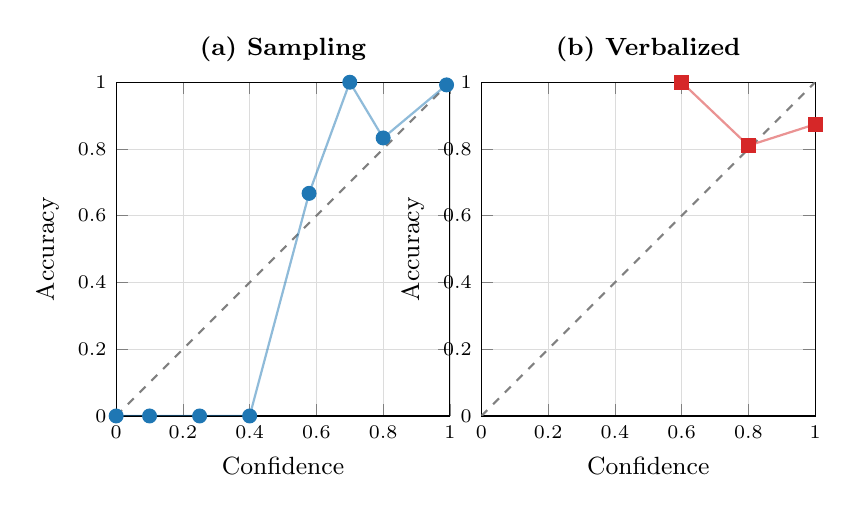
\begin{tikzpicture}
\begin{axis}[
    name=plot1,
    width=0.48\columnwidth,
    height=0.48\columnwidth,
    xlabel={\small Confidence},
    ylabel={\small Accuracy},
    xmin=0, xmax=1,
    ymin=0, ymax=1,
    xtick={0,0.2,0.4,0.6,0.8,1.0},
    ytick={0,0.2,0.4,0.6,0.8,1.0},
    xticklabel style={font=\scriptsize},
    yticklabel style={font=\scriptsize},
    xlabel style={font=\scriptsize},
    ylabel style={font=\scriptsize},
    title={\small (a) Sampling},
    title style={font=\small\bfseries, yshift=-0.5ex},
    grid=major,
    grid style={lightgray, very thin},
    legend style={font=\tiny, at={(0.03,0.97)}, anchor=north west},
]
% Perfect calibration line
\addplot[dashed, gray, thick] coordinates {(0,0) (1,1)};

% Sampling confidence bins (actual data)
\addplot[
    only marks,
    mark=*,
    mark size=2.5pt,
    samplingblue,
    fill=samplingblue,
] coordinates {
    (0.000, 0.000)
    (0.100, 0.000)
    (0.250, 0.000)
    (0.400, 0.000)
    (0.578, 0.667)
    (0.700, 1.000)
    (0.800, 0.833)
    (0.990, 0.992)
};

% Connecting line
\addplot[samplingblue, thick, opacity=0.5] coordinates {
    (0.000, 0.000)
    (0.100, 0.000)
    (0.250, 0.000)
    (0.400, 0.000)
    (0.578, 0.667)
    (0.700, 1.000)
    (0.800, 0.833)
    (0.990, 0.992)
};

\end{axis}

\begin{axis}[
    at={(plot1.east)},
    anchor=west,
    xshift=0.4cm,
    width=0.48\columnwidth,
    height=0.48\columnwidth,
    xlabel={\small Confidence},
    ylabel={\small Accuracy},
    xmin=0, xmax=1,
    ymin=0, ymax=1,
    xtick={0,0.2,0.4,0.6,0.8,1.0},
    ytick={0,0.2,0.4,0.6,0.8,1.0},
    xticklabel style={font=\scriptsize},
    yticklabel style={font=\scriptsize},
    xlabel style={font=\scriptsize},
    ylabel style={font=\scriptsize},
    title={\small (b) Verbalized},
    title style={font=\small\bfseries, yshift=-0.5ex},
    grid=major,
    grid style={lightgray, very thin},
]
% Perfect calibration line
\addplot[dashed, gray, thick] coordinates {(0,0) (1,1)};

% Verbalized confidence bins (actual data)
\addplot[
    only marks,
    mark=square*,
    mark size=2.5pt,
    verbalizedred,
    fill=verbalizedred,
] coordinates {
    (0.600, 1.000)
    (0.800, 0.810)
    (1.000, 0.874)
};

% Connecting line
\addplot[verbalizedred, thick, opacity=0.5] coordinates {
    (0.600, 1.000)
    (0.800, 0.810)
    (1.000, 0.874)
};

\end{axis}
\end{tikzpicture}
\caption{Reliability diagrams on HumanEval. \textbf{(a)}~Sampling confidence closely tracks the diagonal (ECE\,=\,0.021), spanning the full $[0,1]$ range. \textbf{(b)}~Verbalized confidence collapses to only three bins in $[0.6, 1.0]$, with 103 of 164 problems rated at maximum confidence (1.0). The model never rates itself below 0.5.}
\label{fig:reliability}
\end{figure}

The sampling reliability diagram (Figure~\ref{fig:reliability}a) closely follows the diagonal across the full confidence range. Points at low confidence (0.0--0.4) correspond to problems the model consistently fails, and the highest bin (confidence 0.99, accuracy 0.99, $n$\,=\,129) demonstrates that when the model's samples consistently pass, the code is almost always correct.

The verbalized reliability diagram (Figure~\ref{fig:reliability}b) presents a dramatically different picture. Only three bins are populated, all in the range $[0.6, 1.0]$. The model \emph{never} assigns itself a confidence below 0.5, even for problems it gets wrong. The largest bin ($n$\,=\,103) contains problems rated at maximum confidence (1.0), yet the actual accuracy of this bin is only 87.4\%, revealing systematic overconfidence.

\subsection{Confidence Distribution Analysis}

\begin{figure}[t]
\centering
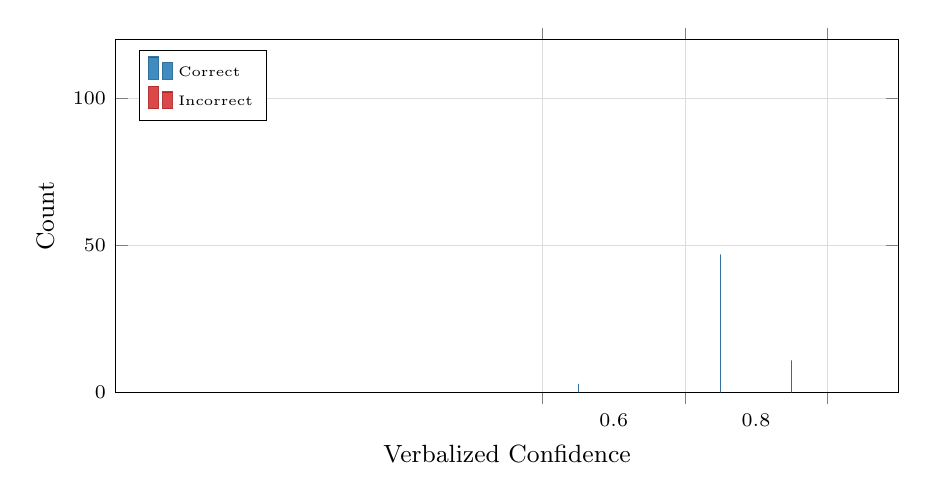
\begin{tikzpicture}
\begin{axis}[
    ybar,
    width=0.95\columnwidth,
    height=0.5\columnwidth,
    xlabel={\small Verbalized Confidence},
    ylabel={\small Count},
    xmin=0, xmax=1.1,
    ymin=0, ymax=120,
    xtick={0.1,0.2,0.3,0.4,0.5,0.6,0.7,0.8,0.9,1.0},
    xticklabel style={font=\scriptsize},
    yticklabel style={font=\scriptsize},
    xlabel style={font=\small},
    ylabel style={font=\small},
    bar width=6pt,
    grid=major,
    grid style={lightgray, very thin},
    ybar interval=0,
    legend style={font=\tiny, at={(0.03,0.97)}, anchor=north west},
    legend cell align={left},
]

% Correct problems (stacked)
\addplot[fill=samplingblue, draw=samplingblue!80!black, opacity=0.85] coordinates {
    (0.6, 3) (0.8, 47) (1.0, 90)
};
\addlegendentry{Correct}

% Incorrect problems
\addplot[fill=verbalizedred, draw=verbalizedred!80!black, opacity=0.85] coordinates {
    (0.6, 0) (0.8, 11) (1.0, 13)
};
\addlegendentry{Incorrect}

\end{axis}
\end{tikzpicture}
\caption{Distribution of verbalized confidence on HumanEval, separated by correctness. The model concentrates its self-assessments in only two bins (0.8 and 1.0) and assigns high confidence to incorrect solutions at nearly the same rate as correct ones. No problem receives a confidence below 0.6.}
\label{fig:distribution}
\end{figure}

Figure~\ref{fig:distribution} shows the distribution of verbalized confidence values on HumanEval, split by correctness. Two features are immediately apparent. First, the distribution is concentrated in only two values: 0.8 ($n$\,=\,58) and 1.0 ($n$\,=\,103), with a negligible number at 0.6 ($n$\,=\,3). The model lacks the vocabulary to express genuine uncertainty. Second, incorrect solutions receive nearly identical confidence distributions to correct ones: 11 of 58 problems at confidence 0.8 are wrong (19.0\%), and 13 of 103 problems at confidence 1.0 are wrong (12.6\%). This confirms that verbalized confidence carries almost no information about correctness (AUROC\,=\,0.546).

\subsection{Cross-Benchmark Consistency}

The MBPP results in Table~\ref{tab:main} confirm that the calibration disconnect is not an artifact of HumanEval. On MBPP, where the model's pass@1 drops to 0.066 due to output format mismatches, the verbalized confidence distribution is nearly identical to HumanEval: 226 of 257 problems receive confidence 0.8, and 29 receive confidence 1.0. The model expresses high confidence on 99.2\% of problems while getting only 6.6\% correct, resulting in catastrophic ECE of 0.755. Meanwhile, sampling confidence correctly identifies the model's poor performance, assigning 229 of 257 problems to the lowest bin (confidence 0.0, accuracy 0.0).

This comparison is particularly revealing because it demonstrates that sampling confidence adapts to the model's actual competence on a given benchmark, while verbalized confidence remains rigidly high regardless of true performance.

% ============================================================
% 5. ANALYSIS & DISCUSSION
% ============================================================
\section{Analysis and Discussion}
\label{sec:discussion}

\subsection{Why Is Verbal Confidence So Poor?}

The disconnect between sampling and verbalized confidence suggests that code LLMs possess reliable internal uncertainty representations but cannot express them through language. We identify three contributing factors.

\paragraph{RLHF incentivizes appearing confident.}
Instruction-tuned models undergo RLHF or similar preference optimization that rewards helpful, confident-sounding responses~\citep{tian2023just}. Human annotators tend to prefer responses that sound authoritative, creating an implicit training signal against expressing uncertainty. This bias is especially pronounced for code, where hedging language (``I'm not sure'') may be penalized even when it would be appropriate.

\paragraph{No training signal for calibrated self-assessment.}
Standard code training pipelines optimize for correctness (pass@1, pass@k) and human preference, but never for the \emph{accuracy of self-reported confidence}. The model has no gradient signal encouraging it to say ``I'm uncertain'' when its internal representations indicate low confidence. The calibrated confidence information exists in the sampling distribution but is never distilled into the model's language generation.

\paragraph{Restricted verbalized confidence vocabulary.}
Our results show that the model effectively uses only two confidence levels (0.8 and 1.0). This extremely coarse discretization cannot capture the rich range of uncertainty present in the sampling distribution, which spans $[0, 1]$ with meaningful variation. The model's language generation has not been trained to produce the linguistic patterns associated with calibrated uncertainty expression.

\subsection{Implications for Coding Agent Design}

Our findings have direct implications for the design of human-centered coding agents.

\paragraph{Leverage sampling, not self-report.}
The near-perfect calibration of sampling confidence (AUROC\,=\,0.990) means that coding agents could provide highly reliable uncertainty signals by generating multiple solutions and computing agreement. Given that generating 10 samples at temperature 0.8 is computationally inexpensive (the entire HumanEval evaluation took approximately 75 minutes on a single GPU), this approach is practical for interactive coding assistants. Agents such as SWE-Agent~\citep{yang2024swe} and OpenHands~\citep{wang2024opendevin} could integrate multi-sample agreement as a lightweight confidence indicator.

\paragraph{Tiered confidence displays.}
The trust calibration literature~\citep{zhang2020effect, yin2019understanding} suggests that well-calibrated confidence can improve human decision-making. A practical coding agent could present confidence as a simple tier (high, medium, low) derived from sampling agreement, with tier boundaries calibrated using reliability diagrams. Based on our data, natural thresholds emerge at pass rates of 0.8 (high), 0.3--0.8 (medium), and below 0.3 (low), which correspond well to the transitions observed in the sampling reliability diagram (Figure~\ref{fig:reliability}a).

\paragraph{Training for calibrated self-report.}
Although self-reported confidence is currently poor, the existence of a strong internal signal provides a training target. Our preliminary SFT experiments (Section~\ref{sec:sft}) suggest that models can be taught to map their sampling consistency to appropriate verbal confidence tiers using execution-labeled training data. Scaling this approach with larger datasets and preference optimization methods such as DPO~\citep{rafailov2023direct} remains a promising direction.

\subsection{Preliminary SFT Results}

We generated 228 confidence-calibrated training pairs from HumanEval using the three-tier scheme described in Section~\ref{sec:sft} and trained a LoRA adapter for 3 epochs. While the small dataset size limits the statistical significance of improvements, the trained model showed qualitative changes in behavior: it began using the target confidence vocabulary and occasionally expressed lower confidence on problems it had previously rated at 1.0. A full-scale evaluation with a larger training set drawn from CodeContests or APPS is needed to quantify calibration improvement, and we leave this to future work.

Our initial DPO training attempt on this dataset produced NaN losses after several hundred steps, consistent with known stability issues when applying DPO to very small preference datasets. Addressing this through dataset scaling, reference model regularization, or alternative preference optimization methods (such as SimPO or KTO) represents a natural next step.

% ============================================================
% 6. LIMITATIONS & FUTURE WORK
% ============================================================
\section{Limitations and Future Work}
\label{sec:limitations}

Our study has several limitations that bound the generality of our claims.

\paragraph{Single model family.}
While we evaluate one model (Qwen2.5-Coder-7B-Instruct) on two benchmarks, extending to additional model families (DeepSeek-Coder~\citep{guo2024deepseek}, CodeLlama, StarCoder) is necessary to establish universality. We note that the calibration disconnect is consistent with findings from \citet{xiong2024can} and \citet{tian2023just} across non-code LLMs, suggesting the phenomenon is general.

\paragraph{Benchmark scope.}
HumanEval and MBPP consist of self-contained function-level problems. Real-world coding tasks involve multi-file edits, integration with existing codebases, and ambiguous specifications~\citep{jimenez2024swe}. Calibration behavior on more complex tasks may differ, and sampling-based confidence becomes more expensive when each sample requires substantial generation.

\paragraph{No human study.}
We do not conduct a user study with developers. While the trust calibration literature~\citep{lee2004trust, yin2019understanding} provides strong theoretical motivation for the value of calibrated confidence, demonstrating actual improvements in developer decision-making requires controlled experiments with professional programmers.

\paragraph{Small SFT dataset.}
Our confidence-calibrated training uses only 228 examples derived from HumanEval, which is insufficient for robust evaluation of the training intervention. Scaling to thousands of examples from diverse coding benchmarks, combined with DPO or GRPO training, is the most important next step.

\paragraph{Verbalized confidence elicitation.}
We use a single prompting strategy (explicit 1--5 scale). Alternative elicitation methods such as chain-of-thought reasoning about difficulty, top-$k$ token probability inspection, or multi-turn self-evaluation may yield different results. \citet{xiong2024can} found that prompting strategy significantly affects verbalized calibration, though no strategy fully closed the gap.

% ============================================================
% 7. CONCLUSION
% ============================================================
\section{Conclusion}
\label{sec:conclusion}

We have measured a striking calibration disconnect in code language models: while sampling-based confidence is near-perfectly calibrated (ECE\,=\,0.021, AUROC\,=\,0.990 on HumanEval), verbalized confidence is essentially random as a correctness predictor (AUROC\,=\,0.546). The model assigns maximum self-rated confidence to 63\% of problems regardless of actual difficulty, and the gap widens to 63$\times$ on MBPP. This disconnect means that code LLMs possess reliable internal uncertainty signals that they cannot communicate through language.

For the growing ecosystem of AI coding agents, this finding is both a problem and an opportunity. The problem is that any agent relying on verbal self-assessment for confidence communication will mislead its users. The opportunity is that sampling-based confidence provides a computationally inexpensive, near-perfectly calibrated alternative that can be integrated into existing agent architectures today.

Bridging the gap between internal and expressed confidence through targeted training on execution-labeled data represents a promising direction for building coding agents that help developers calibrate appropriate trust.

% ============================================================
% ACKNOWLEDGMENTS (suppressed for blind review)
% ============================================================

% ============================================================
% REFERENCES
% ============================================================
\bibliographystyle{icml2026}
\bibliography{references}

\end{document}
